\documentclass[border=6pt]{standalone}
\usepackage{tikz}
\usetikzlibrary{arrows.meta,positioning,calc,shapes.geometric,fit,backgrounds,patterns,matrix,decorations.pathreplacing}
\begin{document}
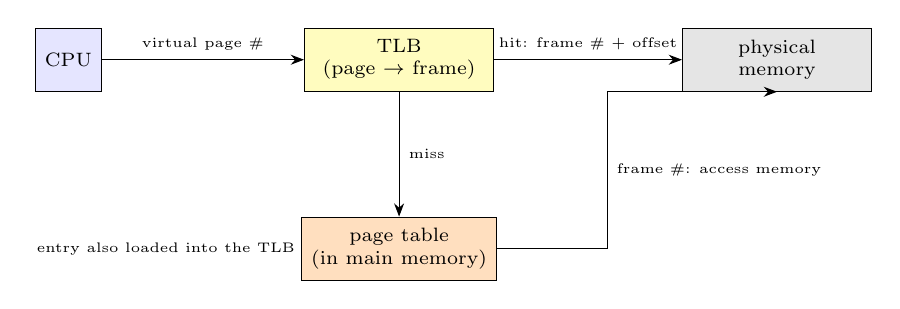
\begin{tikzpicture}[>=Stealth,font=\small]
\tikzstyle{b}=[draw,minimum height=0.8cm,align=center,font=\scriptsize]
\node[b,fill=blue!10] (cpu) at (0,0) {CPU};
\node[b,fill=yellow!25,minimum width=2.4cm] (tlb) at (4.2,0) {TLB\\ (page $\to$ frame)};
\node[b,fill=orange!25,minimum width=2.4cm] (pt) at (4.2,-2.4) {page table\\ (in main memory)};
\node[b,fill=gray!20,minimum width=2.4cm] (mem) at (9.0,0) {physical\\ memory};
\draw[->] (cpu) -- node[above,font=\tiny]{virtual page \#} (tlb);
\draw[->] (tlb) -- node[above,font=\tiny]{hit: frame \# + offset} (mem);
\draw[->] (tlb.south) -- node[right,font=\tiny]{miss} (pt.north);
\draw[->] (pt.east) -- ++(1.4,0) |- node[pos=0.25,right,font=\tiny]{frame \#: access memory} (mem.south);
\node[font=\tiny,anchor=east] at (3.0,-2.4) {entry also loaded into the TLB};
\end{tikzpicture}
\end{document}
